\subsection{Latch SR}

O latch SR (Set-Reset) é o elemento de memória mais simples, composto por duas portas lógicas interligadas por realimentação.

Ele possui duas entradas principais:
\begin{itemize}
    \item $S$ (Set): força a saída para 1
    \item $R$ (Reset): força a saída para 0
\end{itemize}

Seu comportamento pode ser descrito pela seguinte tabela de transição de estados:

\begin{center}
\begin{tabular}{c c | c}
S & R & $Q_{t+1}$ \\
\hline
0 & 0 & $Q_t$ \\
0 & 1 & 0 \\
1 & 0 & 1 \\
1 & 1 & indefinido
\end{tabular}
\end{center}

onde $Q_t$ representa o estado atual e $Q_{t+1}$ o próximo estado do sistema.

Observa-se que, na ausência de estímulos ($S = R = 0$), o circuito preserva seu estado anterior. Essa propriedade de retenção de informação caracteriza um elemento de memória.

Existem duas implementações clássicas do latch SR, baseadas em portas NOR e NAND:

\begin{figure}[H]
    \centering
    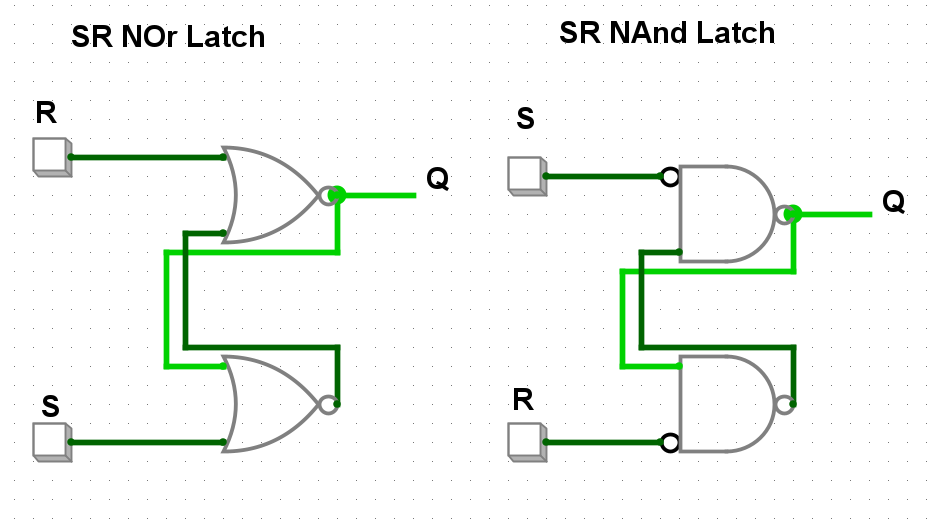
\includegraphics[width=0.6\linewidth]{images/sr-latch-circuit.png}
    \caption{Implementações do latch SR com portas NOR e NAND}
    \label{fig:sr-latch-circuit}
\end{figure}

Neste trabalho, será utilizada a implementação com portas NOR.

Utilizando redstone, é possível construir um latch SR equivalente:

\begin{figure}[H]
    \centering
    \includegraphics[width=0.8\linewidth]{images/sr-nor-latch-redstone.png}
    \caption{Latch SR implementado no Minecraft}
    \label{fig:sr-nor-latch-redstone}
\end{figure}

A condição $S = R = 1$ é considerada inválida pois força simultaneamente as duas saídas do circuito, violando a relação complementar entre $Q$ e $\lnot Q$. Em circuitos reais, isso pode levar a um estado indeterminado ou metaestável, no qual o valor final não é previsível.

Pode-se adicionar um controle de clock a partir de duas portas AND, recebendo as entradas $S$ e $R$ e o pulso de clock.

\begin{figure}[H]
    \centering
    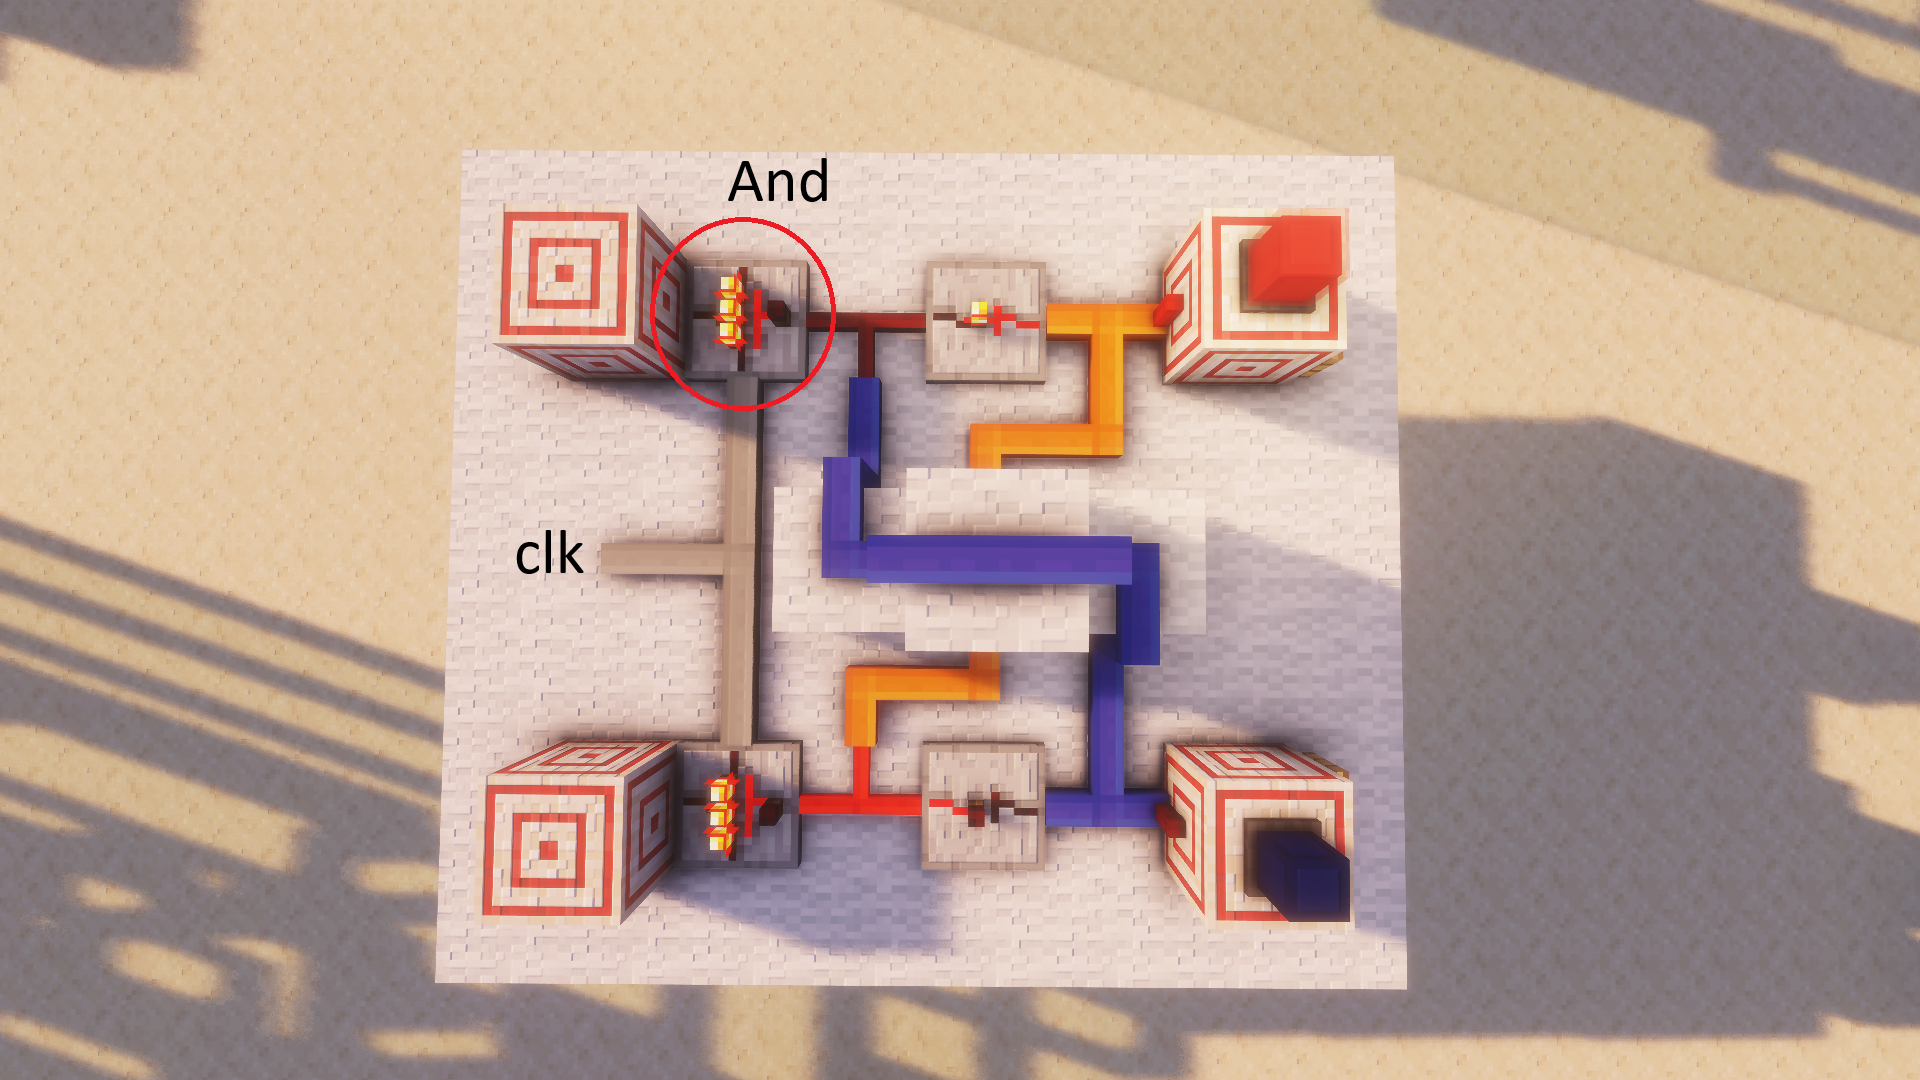
\includegraphics[width=0.8\linewidth]{images/sr-nor-latch-redstone-clock.png}
    \caption{Latch SR implementado no Minecraft com controle de clock}
    \label{fig:sr-nor-latch-redstone-clock}
\end{figure}